% ============================================================
%  DISCOVERY CURRICULUM — Journey 1, Module 1
%  "Numbers as Descriptions of Reality"
%  Compile with: pdflatex J1_M1.tex  (run twice for references)
% ============================================================

\documentclass[12pt, a4paper]{article}

\usepackage[a4paper, top=2.8cm, bottom=2.8cm, left=3.0cm, right=2.5cm, includeheadfoot, headheight=15pt]{geometry}
\usepackage{amsmath, amsthm}
\usepackage[charter, cal=cmcal]{mathdesign}
\usepackage[scaled=0.92]{helvet}
\usepackage{xcolor}
\usepackage{tcolorbox}
\tcbuselibrary{skins, breakable, theorems}
\usepackage{enumitem}
\usepackage{graphicx}
\usepackage{tikz}
\usetikzlibrary{arrows.meta, positioning, calc}
\usepackage{pgfplots}
\pgfplotsset{compat=1.18}
\usepackage{booktabs}
\usepackage{array}
\usepackage{fancyhdr}
\usepackage{titlesec}
\usepackage{parskip}
\usepackage{microtype}
\usepackage{hyperref}
\hypersetup{colorlinks=true, linkcolor=NavyBlue, urlcolor=NavyBlue}

% ── Colours ─────────────────────────────────────────────────
\definecolor{NavyBlue}{HTML}{1E3A8A}
\definecolor{MidBlue}{HTML}{2E6DA4}
\definecolor{Gold}{HTML}{D97706}
\definecolor{LightBlue}{HTML}{EFF6FF}
\definecolor{LightGold}{HTML}{FEF3C7}
\definecolor{DarkGrey}{HTML}{334155}
\definecolor{BoxGreen}{HTML}{F0FDF4}
\definecolor{SoftRed}{HTML}{FFF1F2}
\definecolor{SidebarGrey}{HTML}{F8FAFC}

% ── Section formatting ───────────────────────────────────────
\titleformat{\section}{\Large\bfseries\color{NavyBlue}}{}{0em}{}[{\color{MidBlue}\vspace{2pt}\rule{\linewidth}{1.5pt}}]
\titleformat{\subsection}{\large\bfseries\color{MidBlue}}{}{0em}{}
\titleformat{\subsubsection}{\normalsize\bfseries\color{Gold}}{}{0em}{}

% ── Header / Footer ─────────────────────────────────────────
\pagestyle{fancy}
\fancyhf{}
\fancyhead[L]{\small\color{DarkGrey}\textit{Discovery Curriculum}}
\fancyhead[R]{\small\color{DarkGrey}\textit{Journey 1 $\cdot$ Module 1}}
\fancyfoot[C]{\small\color{MidBlue}\thepage}
\renewcommand{\headrulewidth}{0.4pt}

% ── Environments (tcolorbox Unification) ─────────────────────

% Puzzle box — opening problem
\newtcolorbox{puzzlebox}[1][]{
  enhanced, breakable,
  colback=NavyBlue!5, colframe=NavyBlue,
  boxrule=0pt, leftrule=2.5pt,
  sharp corners,
  left=12pt, right=10pt, top=10pt, bottom=10pt,
  before skip=14pt, after skip=10pt,
  #1
}

% Discovery box — moment of crystallisation
\newtcolorbox{discoverybox}[1][]{
  enhanced, breakable,
  colback=LightGold, colframe=Gold,
  boxrule=0pt, leftrule=2.5pt,
  sharp corners,
  left=12pt, right=10pt, top=10pt, bottom=10pt,
  before skip=14pt, after skip=10pt,
  #1
}

% Name box — formal definition reveal
\newtcolorbox{namebox}[1][]{
  enhanced, breakable,
  colback=LightBlue, colframe=MidBlue,
  boxrule=0.8pt,
  arc=4pt,
  left=12pt, right=10pt, top=10pt, bottom=10pt,
  before skip=14pt, after skip=10pt,
  #1
}

% Reflection box
\newtcolorbox{reflectionbox}[1][]{
  enhanced, breakable,
  colback=BoxGreen, colframe=DarkGrey!35,
  boxrule=0.8pt,
  arc=4pt,
  left=12pt, right=10pt, top=10pt, bottom=10pt,
  before skip=14pt, after skip=10pt,
  #1
}

% Thought provocation — inline philosophical aside
\newtcolorbox{thought}[1][]{
  enhanced, breakable,
  colback=SidebarGrey, colframe=Gold,
  boxrule=0pt, leftrule=1.5pt,
  sharp corners,
  left=10pt, right=10pt, top=7pt, bottom=7pt,
  before skip=10pt, after skip=10pt,
  #1
}

% Problem counter
\newcounter{problem}
\newenvironment{problem}[1][]{%
  \refstepcounter{problem}%
  \par\vspace{6pt}%
  \noindent\textbf{\color{MidBlue}Problem \theproblem}%
  \ifx&#1&\else\ \textit{(#1)}\fi\textbf{.}\enskip
}{\par\vspace{4pt}}

% Deep problem counter
\newcounter{deepproblem}
\newenvironment{deepproblem}[1][]{%
  \refstepcounter{deepproblem}%
  \par\vspace{6pt}%
  \noindent\textbf{\color{NavyBlue}$\bigstar$\ Deep Problem \thedeepproblem}%
  \ifx&#1&\else\ \textit{(#1)}\fi\textbf{.}\enskip
}{\par\vspace{4pt}}

% Exercise counter
\newcounter{exercise}
\newenvironment{exercise}[1][]{%
  \refstepcounter{exercise}%
  \par\vspace{6pt}%
  \noindent\textbf{\color{Gold}Exercise \theexercise}%
  \ifx&#1&\else\ \textit{(#1)}\fi\textbf{.}\enskip
}{\par\vspace{4pt}}



% ============================================================
\begin{document}
% ============================================================

% ── Cover ───────────────────────────────────────────────────
\thispagestyle{empty}
\begin{center}
{\small\color{MidBlue}\textbf{DISCOVERY CURRICULUM}\quad$\cdot$\quad\textbf{JOURNEY 1: REPRESENTATION}}

\vspace{0.6cm}
{\color{NavyBlue}\rule{\linewidth}{2pt}}
\vspace{0.5cm}

{\Huge\bfseries\color{NavyBlue}Module 1}\\[0.3cm]
{\LARGE\bfseries\color{MidBlue}Numbers as Descriptions of Reality}\\[0.4cm]
{\color{Gold}\rule{0.4\linewidth}{1.2pt}}\\[0.4cm]
{\large\itshape\color{DarkGrey}How does mathematics reach out and grab hold of the world?\\[0.15cm]
And how tightly does it actually hold?}

\vspace{1cm}
\begin{tabular}{rl}
\color{DarkGrey}\textbf{Journey}           & Journey 1 --- Representation \\[4pt]
\color{DarkGrey}\textbf{Module}            & 1 of 6 \\[4pt]
\color{DarkGrey}\textbf{Prerequisites}     & Olympiad algebra, basic combinatorics \\[4pt]
\color{DarkGrey}\textbf{You will discover} & Functions, domain, codomain, composition \\[4pt]
\color{DarkGrey}\textbf{Format}            & 8 problems $+$ 3 deep problems $\approx$ 12--14 pages \\
\end{tabular}

\vspace{1cm}
{\color{NavyBlue}\rule{\linewidth}{2pt}}
\end{center}

\newpage


% ============================================================
\section{Part 1 \texorpdfstring{---}{--} The Puzzle}
% ============================================================

\begin{puzzlebox}
\textbf{The Opening Puzzle.}

You are standing by the side of a road. A car passes you and drives away into the distance. A friend turns to you and asks: \textit{``How far away is the car right now?''}

You glance at your watch. Five seconds have passed since the car went by. The car has been moving at a steady speed the whole time.

\medskip
\textbf{Question.} What information would you need to answer your friend's question precisely? And can you write a single rule --- not a sentence, but a mathematical expression --- that gives the distance for \emph{any} amount of time that might have elapsed?
\end{puzzlebox}

\medskip
Most people, when they read this, immediately reach for a formula. That instinct --- to compress a situation into a symbol --- is one of the most powerful things the human mind does. It is also, if you examine it carefully, a genuinely strange thing to do.

Think about what you are actually attempting. The car is a physical object. It has weight, colour, a specific engine. The road has cracks in it. The air has resistance. The driver might brake. None of that is in your formula. When you write $d = 15t$, you have replaced a rich, messy, particular situation with a clean, general, abstract one. You have performed an act of \emph{idealisation}.

\begin{thought}
\textbf{Worth pausing on.} When a physicist writes an equation for a falling object, they assume the object is a perfect point mass, that gravity is constant, that there is no air. Real objects are not point masses. Real gravity varies. Real air exists. The equation is not the world --- it is a \emph{model} of the world, carefully stripped of everything that would make it complicated. The power of the model comes precisely from what it throws away.

This is not a flaw. It is a design choice. The question mathematicians and scientists are always asking is: \textit{what can I safely ignore, and what must I keep?}
\end{thought}

\medskip
What you just tried to write is one of the most fundamental objects in all of mathematics. We will spend this module understanding what it really is.

% ============================================================
\section{Part 2 \texorpdfstring{---}{--} Exploration}
% ============================================================

We approach the puzzle through eight smaller problems. Each one is designed to surface something you already implicitly know --- something you have been using without ever naming.

\subsection{Step 1: The act of describing}

\begin{problem}
\label{prob:car}
Here is a table of observations about the car from the puzzle.

\begin{center}
\begin{tabular}{cc}
\toprule
\textbf{Time elapsed (seconds)} & \textbf{Distance from you (metres)} \\
\midrule
0 & 0 \\
1 & 15 \\
2 & 30 \\
3 & 45 \\
4 & 60 \\
\bottomrule
\end{tabular}
\end{center}

\begin{enumerate}[label=(\alph*), topsep=2pt]
  \item What pattern do you see in the numbers?
  \item Write a rule using $t$ (time in seconds) and $d$ (distance in metres) that captures this pattern.
  \item Use your rule to predict the distance at $t = 7$ seconds. At $t = 100$ seconds.
  \item Does your rule work for $t = 0.5$? For $t = -1$? What would a negative value of $t$ even mean here?
  \item Does your rule work for $t = 10{,}000$? For $t = 1{,}000{,}000$? Be honest: at what point does the model break down as a description of the real car?
\end{enumerate}
\end{problem}

\medskip
Notice what you did in part (b). You introduced two letters, $t$ and $d$, and wrote a relationship between them. Those letters are called \textbf{variables} --- but this word deserves more scrutiny than it usually gets.

\begin{thought}
\textbf{What is a variable, really?}
A variable is a \emph{placeholder} --- a symbol that stands in for any value from some collection of possibilities. When you write $t$, you do not mean a specific number. You mean: \textit{whatever time we happen to be asking about.} The variable is a way of making a statement that is simultaneously true for infinitely many particular cases. This is the beginning of abstraction. Instead of saying ``at 3 seconds the car is 45 metres away,'' you say something that is true for all seconds at once.

Abstraction is not vagueness. It is precision applied to a whole class of situations at once. It is one of the central acts of mathematical thought.
\end{thought}

\begin{problem}
Consider a square with side length $s$.
\begin{enumerate}[label=(\alph*), topsep=2pt]
  \item Write a rule connecting $s$ to the area $A$ of the square.
  \item Write a rule connecting $s$ to the perimeter $P$.
  \item Find a rule connecting $A$ directly to $P$, eliminating $s$ entirely.
  \item If someone tells you $A = 36$, can you determine $P$? Is there only one answer?
  \item Draw a square with side length 1 on paper. Now measure it with a ruler. Is the area exactly 1? Reflect on what your measurement tells you about the difference between geometric objects and physical ones.
\end{enumerate}
\end{problem}

Part (e) of Problem~2 points at something profound. The rule $A = s^2$ is exactly, perfectly, permanently true --- but only for an ideal mathematical square. A square drawn with a pencil has rounded corners, imperfect sides, a thickness to its lines. The equation does not describe that square. It describes a \emph{concept} of a square.

\begin{thought}
\textbf{The gap between model and reality.}
Geometry began as a practical tool for measuring land, building pyramids, navigating by stars. But the objects of geometry --- perfect points, infinitely thin lines, ideal circles --- do not exist in the physical world. No one has ever held a perfect triangle. In this sense, mathematics is always a slight lie: a beautiful, useful, controllable lie that we tell about the world in order to reason about it clearly. The extraordinary thing is how well it works.
\end{thought}

\begin{problem}
A taxi charges a fixed fee of 50 KES to start, then 12 KES per kilometre.
\begin{enumerate}[label=(\alph*), topsep=2pt]
  \item Write a rule connecting distance $x$ (km) to total fare $F$ (KES).
  \item What is the fare for a 7~km journey? For a 0~km journey?
  \item A passenger pays 194 KES. How far did they travel?
  \item Can the fare ever be negative? What does this tell us about which values of $x$ make physical sense?
  \item The rule assumes the price per kilometre is constant. List three real-world factors that would make this assumption false.
\end{enumerate}
\end{problem}

\subsection{Step 2: When one thing determines another}

These three problems all share a hidden structure. Let us bring it into the open.

In each case:
\begin{itemize}[topsep=4pt]
  \item There is an \textbf{input} quantity --- time, side length, distance travelled.
  \item There is an \textbf{output} quantity --- distance, area, fare.
  \item There is a \textbf{rule} that turns any input into a specific output.
\end{itemize}

That last condition --- \emph{one specific output per input} --- is more important than it sounds. Let us test it.

\begin{problem}
\label{prob:oneoutput}
For each rule below, ask: does every input give \emph{exactly one} output?
\begin{enumerate}[label=(\alph*), topsep=2pt]
  \item ``The output is the square of the input.'' \hfill ($y = x^2$)
  \item ``The output is a number whose square equals the input.'' \hfill (find $y$ where $y^2 = x$)
  \item ``The output is the day of the week on which the input date falls.''
  \item ``The output is a prime factor of the input.''
  \item ``The output is the number of letters in the English spelling of the input.'' \hfill (inputs: 1, 2, 3, \ldots)
\end{enumerate}
For the ambiguous cases: what exactly goes wrong?
\end{problem}

\begin{discoverybox}
\textbf{Pause and notice.}

Some rules in Problem~\ref{prob:oneoutput} are \emph{reliable}: one input, one definite output, every time. Others are \emph{ambiguous}: one input can give multiple different outputs.

This difference is not a technicality. Mathematics requires reliable rules. An ambiguous rule is a \emph{relationship} between quantities, but it is not a functional one. It does not let you make predictions. It does not let you substitute and compute.

\medskip
\textbf{Before reading on:} in your own words, write down what a ``reliable rule'' means. What is the exact condition that separates a reliable rule from an ambiguous one?
\end{discoverybox}

\subsection{Step 3: Where rules stop working}

\begin{problem}
Consider the rule $\displaystyle y = \dfrac{1}{x}$.
\begin{enumerate}[label=(\alph*), topsep=2pt]
  \item Compute $y$ for $x = 1,\; 2,\; 0.5,\; 0.1,\; 0.01,\; 0.001$.
  \item What happens as $x$ gets closer and closer to zero?
  \item What happens \emph{at} $x = 0$ exactly?
  \item Compute $y$ for $x = -1,\; -2,\; -0.5$.
  \item Sketch the behaviour of this rule. (Rough is fine --- capture the essential shape.)
\end{enumerate}
\end{problem}

\begin{center}
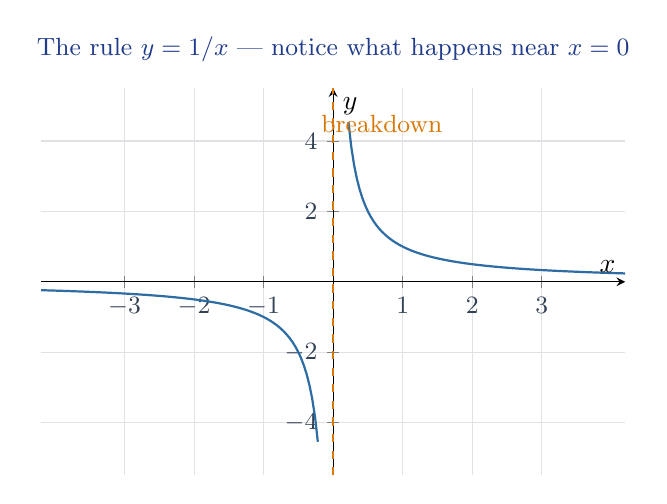
\begin{tikzpicture}
\begin{axis}[
  width=9cm, height=6.5cm,
  axis lines=center,
  xlabel={$x$}, ylabel={$y$},
  xmin=-4.2, xmax=4.2, ymin=-5.5, ymax=5.5,
  xtick={-3,-2,-1,1,2,3}, ytick={-4,-2,2,4},
  tick label style={font=\small, color=DarkGrey},
  grid=major, grid style={DarkGrey!15},
  title={\small\color{NavyBlue} The rule $y = 1/x$ --- notice what happens near $x = 0$},
]
\addplot[MidBlue, thick, domain=-4.2:-0.22, samples=100] {1/x};
\addplot[MidBlue, thick, domain=0.22:4.2, samples=100] {1/x};
\addplot[Gold, dashed, thick] coordinates {(0,-5.5)(0,5.5)};
\node[color=Gold, font=\small] at (axis cs:0.7, 4.5) {breakdown};
\end{axis}
\end{tikzpicture}
\end{center}

\begin{thought}
\textbf{Division by zero.}
The failure of $y = 1/x$ at $x = 0$ is not just a quirk. It is telling you something deep: not every rule works everywhere. Every rule has a natural \emph{territory} --- a set of inputs on which it behaves. Outside that territory, the rule either gives nonsense, or ceases to be a rule at all. Recognising the territory of a rule is as important as knowing the rule itself. Much of analysis --- one of the great branches of mathematics --- is the study of where and how functions break down.
\end{thought}

\begin{problem}
\label{prob:population}
The population $P$ (in millions) of a city is modelled by
\[
  P(t) \;=\; 2 \cdot (1.05)^{t},
\]
where $t$ is years since the year 2000.
\begin{enumerate}[label=(\alph*), topsep=2pt]
  \item What was the population in 2000? In 2010?
  \item When does the population first exceed 4 million? (Experiment with values of $t$, or think carefully.)
  \item What does $P(-10)$ represent? Compute it. Does the answer make sense?
  \item This model predicts the population for $t = 500$. Compute it. Comment.
  \item Suggest two real-world events that could make this model completely wrong.
\end{enumerate}
\end{problem}

Problems~5 and~6 together illustrate a key tension. Mathematically, $P(t) = 2 \cdot (1.05)^t$ is perfectly well-defined for any real number $t$ --- including $t = 10^9$. But physically, the rule tells us nothing useful for large $t$. The mathematics and the reality have parted ways.

\begin{thought}
\textbf{The model is not the thing.}
A map is useful precisely because it is not the territory. If a map showed every pebble, every tree, every crack in the pavement, it would be useless --- you would need the territory to read the map. But a map that is too simplified --- that shows only one road in a city of ten thousand --- is also useless. The art of modelling is deciding how much to simplify. Too much, and you lose the truth. Too little, and you lose the power of mathematics.

This is not a solved problem. Scientists and mathematicians argue constantly about whether a given model is faithful enough to reality to be trusted.
\end{thought}

\subsection{Step 4: Building rules from rules}

\begin{problem}
\label{prob:factory}
A factory converts raw material (in kg) to product (in units) at a rate of 3 units per kg. Each unit sells for 25 KES.
\begin{enumerate}[label=(\alph*), topsep=2pt]
  \item Write a rule $U(m)$ giving the number of units produced from $m$ kg.
  \item Write a rule $R(u)$ giving the revenue from selling $u$ units.
  \item Write a single rule $T(m)$ giving total revenue from $m$ kg, without using $u$.
  \item How did you build $T$ from $U$ and $R$? Describe the process precisely, in words.
\end{enumerate}
\end{problem}

\begin{problem}
Let $f(x) = x^2 + 1$ and $g(x) = 2x - 3$.
\begin{enumerate}[label=(\alph*), topsep=2pt]
  \item Compute $f(g(2))$. Compute $g(f(2))$. Are they equal?
  \item Write a formula for $f(g(x))$: substitute the entire expression $2x-3$ wherever $f$ uses $x$.
  \item Write a formula for $g(f(x))$.
  \item If $h(x) = f(g(x))$, compute $h(5)$. Verify by computing $g(5)$ first, then applying $f$.
  \item Does composition behave like multiplication? That is: is $f \circ g$ always the same as $g \circ f$?
\end{enumerate}
\end{problem}

What you built in Problems~\ref{prob:factory} and~8 is called the \textbf{composition} of two rules: the output of one becomes the input of the next. This operation --- chaining rules together --- is one of the most powerful ideas in mathematics. It reappears in derivatives, in transforms, in algorithms, in the definition of continuity, in category theory.

% ============================================================
\section{Part 3 \texorpdfstring{---}{--} Discovery}
% ============================================================

\begin{discoverybox}
\textbf{What have we built?}

Look back over all eight problems. Each one involved the same underlying structure:

\begin{enumerate}
  \item A set of permitted \textbf{inputs}.
  \item A \textbf{rule} assigning to each input \emph{exactly one} output.
  \item A set of possible \textbf{outputs}.
\end{enumerate}

This three-part structure --- with the guarantee of exactly one output per input --- is one of the foundational objects of all mathematics. It appears inside derivatives, inside probability distributions, inside the definition of a matrix, inside quantum mechanics.

\medskip
\textbf{Before reading on:} write your own name and your own definition for this object. Then compare it with the one in the next section.
\end{discoverybox}

% ============================================================
\section{Part 4 \texorpdfstring{---}{--} Naming the Idea}
% ============================================================

\begin{namebox}
\textbf{What mathematicians call it: a \emph{function}.}

The object you have been working with is called a \textbf{function}. The terminology was standardised over the 17th--19th centuries. \textbf{Gottfried Wilhelm Leibniz} (1646--1716) used the word early on. \textbf{Leonhard Euler} (1707--1783) introduced the compact notation $f(x)$. \textbf{Peter Dirichlet} (1805--1859) gave the definition now used in modern mathematics.

\medskip
Formally, a \textbf{function} $f$ from a set $A$ to a set $B$ is a rule assigning to each element $a \in A$ exactly one element $f(a) \in B$:
\[
  f : A \longrightarrow B, \qquad a \;\longmapsto\; f(a).
\]

\begin{itemize}[topsep=4pt]
  \item $A$ is the \textbf{domain} --- the set of permitted inputs.
  \item $B$ is the \textbf{codomain} --- the set of possible outputs.
  \item $f(A) = \{\, f(a) : a \in A \,\}$ is the \textbf{range} (or \textbf{image}) --- the outputs actually achieved.
\end{itemize}

\begin{center}
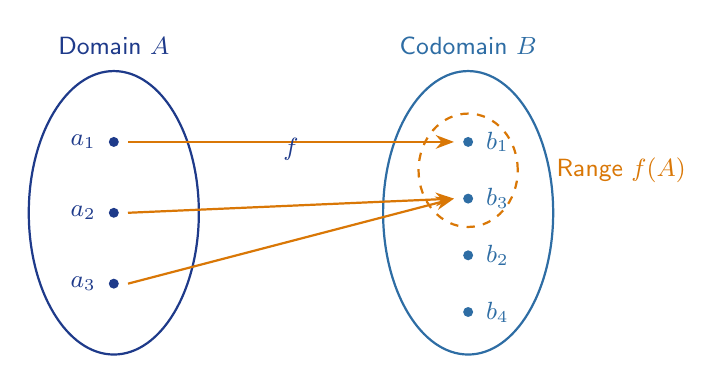
\begin{tikzpicture}[scale=0.9, >=Stealth, every node/.style={font=\sffamily\small}]
  % Set A (Domain)
  \draw[thick, NavyBlue] (-2.5,0) ellipse (1.2cm and 2cm);
  \node[NavyBlue, above] at (-2.5,2.1) {Domain $A$};
  
  \fill[NavyBlue] (-2.5,1.0) circle (2pt) node[left=3pt] {$a_1$};
  \fill[NavyBlue] (-2.5,0.0) circle (2pt) node[left=3pt] {$a_2$};
  \fill[NavyBlue] (-2.5,-1.0) circle (2pt) node[left=3pt] {$a_3$};

  % Set B (Codomain)
  \draw[thick, MidBlue] (2.5,0) ellipse (1.2cm and 2cm);
  \node[MidBlue, above] at (2.5,2.1) {Codomain $B$};

  \fill[MidBlue] (2.5,1.0) circle (2pt) node[right=3pt] {$b_1$};
  \fill[MidBlue] (2.5,0.2) circle (2pt) node[right=3pt] {$b_3$};
  \fill[MidBlue] (2.5,-0.6) circle (2pt) node[right=3pt] {$b_2$};
  \fill[MidBlue] (2.5,-1.4) circle (2pt) node[right=3pt] {$b_4$};

  % Range subset (dashed ellipse enclosing b1 and b3)
  \draw[dashed, Gold, thick] (2.5,0.6) ellipse (0.7cm and 0.8cm);
  \node[Gold, right=1.0cm] at (2.5,0.6) {Range $f(A)$};

  % Mapping arrows
  \draw[->, thick, Gold] (-2.3, 1.0) -- (2.3, 1.0);
  \draw[->, thick, Gold] (-2.3, 0.0) -- (2.3, 0.2);
  \draw[->, thick, Gold] (-2.3, -1.0) -- (2.3, 0.2);

  % Function label
  \node[above] at (0, 0.6) {\textcolor{NavyBlue}{$f$}};
\end{tikzpicture}
\end{center}


The requirement ``exactly one output per input'' is what separates a \emph{function} from a general \emph{relation} between sets.

\medskip
\textbf{Composition.} If $f : A \to B$ and $g : B \to C$, the composition
\[
  g \circ f \;:\; A \to C, \qquad (g \circ f)(a) = g(f(a))
\]
is itself a function. Observe: the codomain of $f$ must match the domain of $g$ for composition to be defined. Types must fit.
\end{namebox}

\medskip
\noindent\textbf{Why does this matter?}
Functions are the basic vocabulary of all the mathematics ahead. Derivatives are functions. Integrals produce functions from functions. A probability distribution is a function. A matrix acting on a vector is a function. The Fourier transform is a function that takes functions as input and returns functions as output. Once you own the idea of a function deeply, the rest of the curriculum makes sense in a way that it simply cannot if you think of functions as just ``formulas with $x$ in them.''

\begin{thought}
\textbf{From particular to general.}
The car problem at the start of this module was about one specific car, on one specific road, on one specific day. The function $d(t) = 15t$ is about all cars travelling at 15 m/s, everywhere, for all time. By moving from the particular to the general, we gained enormous power: a single statement captures infinitely many situations. This is what abstraction \emph{does}. It is not about being vague. It is about being maximally efficient with truth.
\end{thought}

% ============================================================
\section{Part 5 \texorpdfstring{---}{--} Solved Exercises}
% ============================================================

These short, direct exercises are designed to help you get comfortable with the vocabulary, notations, and basic operations of functions. Work through them and compare your answers with the solutions provided.

\begin{exercise}[Evaluating and Equating Functions]
Let $f(x) = x^2 - 4x + 3$. Find all real numbers $x$ such that $f(x) = f(2 - x)$.
\end{exercise}

\textbf{Solution.}
We expand the expression for $f(2 - x)$ by substituting $(2-x)$ in place of $x$:
\[
  f(2 - x) \;=\; (2 - x)^2 - 4(2 - x) + 3
\]
Expanding the terms:
\[
  f(2 - x) \;=\; (4 - 4x + x^2) - (8 - 4x) + 3 \;=\; x^2 - 1.
\]
Now we set $f(x) = f(2 - x)$:
\[
  x^2 - 4x + 3 \;=\; x^2 - 1.
\]
Subtracting $x^2$ from both sides:
\[
  -4x + 3 \;=\; -1 \implies -4x \;=\; -4 \implies x \;=\; 1.
\]
Thus, the only real number satisfying the condition is $x = 1$.

\begin{exercise}[Finding Domain and Range]
Let $f(x) = \sqrt{9 - x^2}$ be a real-valued function. Find its largest possible domain $A \subseteq \mathbb{R}$ and its corresponding range $f(A)$.
\end{exercise}

\textbf{Solution.}
For $f(x)$ to yield a real value, the expression inside the square root must be non-negative:
\[
  9 - x^2 \;\ge\; 0 \implies x^2 \;\le\; 9 \implies -3 \;\le\; x \;\le\; 3.
\]
Thus, the largest possible domain is $A = [-3, 3]$. 

For the range, as $x$ varies over $[-3, 3]$, the term $x^2$ spans the interval $[0, 9]$. Consequently:
\[
  9 - x^2 \;\in\; [0, 9].
\]
Taking the principal square root:
\[
  \sqrt{9 - x^2} \;\in\; [0, 3].
\]
Thus, the range of the function is $f(A) = [0, 3]$.

\begin{exercise}[Function Composition and Domains]
Let $f(x) = \dfrac{x}{x-1}$ defined for all real $x \neq 1$. Show that the composition $(f \circ f)(x) = x$ and specify the domain of this composition.
\end{exercise}

\textbf{Solution.}
We compute the composite function $(f \circ f)(x) = f(f(x))$:
\[
  f(f(x)) \;=\; f\left(\dfrac{x}{x-1}\right) \;=\; \dfrac{\dfrac{x}{x-1}}{\dfrac{x}{x-1} - 1}.
\]
Simplifying the denominator:
\[
  \dfrac{x}{x-1} - 1 \;=\; \dfrac{x - (x - 1)}{x - 1} \;=\; \dfrac{1}{x - 1}.
\]
Substituting this back:
\[
  f(f(x)) \;=\; \dfrac{\dfrac{x}{x-1}}{\dfrac{1}{x-1}} \;=\; x.
\]
For the composite function $f(f(x))$ to be defined, two conditions must hold:
1. $x$ must be in the domain of the inner function $f$, which requires $x \neq 1$.
2. $f(x)$ must be in the domain of the outer function $f$, which requires $f(x) \neq 1$.

Let us check if $f(x)$ can ever equal $1$:
\[
  \dfrac{x}{x-1} \;=\; 1 \implies x \;=\; x - 1 \implies 0 \;=\; -1.
\]
This equation has no solution. Thus, $f(x)$ is never $1$. 

The domain of the composition $f \circ f$ is therefore all real numbers except $1$, i.e., $\mathbb{R} \setminus \{1\}$, even though the simplified expression is just $x$.

\bigskip

% ============================================================
\section{Part 6 \texorpdfstring{---}{--} Problems}
% ============================================================

These problems require conceptual synthesis and a deeper level of logical deduction. Use them to establish a firm foothold on functional reasoning.

\begin{problem}[Fixed Points of Commuting Functions]
Let $f : S \to S$ and $g : S \to S$ be functions that commute under composition, meaning $f \circ g = g \circ f$. A point $x_0 \in S$ is a \emph{fixed point} of $f$ if $f(x_0) = x_0$. Prove that if $f$ has a unique fixed point $x_0$, then $x_0$ must also be a fixed point of $g$.
\end{problem}

\begin{problem}[Involutions and Monotonicity]
A function $f : \mathbb{R} \to \mathbb{R}$ is called an \emph{involution} if $f(f(x)) = x$ for all $x \in \mathbb{R}$. Prove that if $f$ is an involution and is strictly increasing, then $f(x) = x$ for all $x \in \mathbb{R}$.
\end{problem}

\begin{problem}[Constructing Bijections]
Let $A$ and $B$ be finite sets.
\begin{enumerate}[label=(\alph*)]
  \item Prove that there exists a bijection between the Cartesian products $A \times B$ and $B \times A$.
  \item If $|A| = m$ and $|B| = n$, prove by induction or combinatorial counting that the total number of functions from $A$ to $B$ is $n^m$.
\end{enumerate}
\end{problem}

\bigskip

% ============================================================
\section{Part 7 \texorpdfstring{---}{--} Deep Problems}
% ============================================================

These problems are harder. Some will require sustained thought over hours or days. That is expected. Write down partial progress. Return to them.

\begin{deepproblem}[Cauchy's Functional Equation]
A function $f : \mathbb{R} \to \mathbb{R}$ satisfies the rule
\[
  f(x + y) \;=\; f(x) + f(y) \quad \text{for all } x, y \in \mathbb{R}.
\]
\begin{enumerate}[label=(\alph*)]
  \item Prove that $f(0) = 0$.
  \item Prove that $f(-x) = -f(x)$ for all $x$.
  \item Prove that $f(nx) = n\,f(x)$ for all integers $n$.
  \item Prove that $f(rx) = r\,f(x)$ for all rational numbers $r$.
  \item Assuming $f$ is continuous, prove that $f(x) = cx$ for some constant $c \in \mathbb{R}$. \textit{Hint: let $c = f(1)$, then use the rational case and continuity to extend to all reals.}
  \item \textit{(Challenge.)} If $f$ is not assumed continuous, the conclusion $f(x) = cx$ can fail spectacularly. Can you explain, without constructing one explicitly, why such pathological functions must exist? What does their existence say about the relationship between algebra and topology?
\end{enumerate}
\end{deepproblem}

\begin{deepproblem}[Injectivity and Surjectivity]
Let $f : A \to B$ be a function.
\begin{enumerate}[label=(\alph*)]
  \item $f$ is \textbf{injective} (one-to-one) if $f(a_1) = f(a_2)$ implies $a_1 = a_2$. Explain this in plain language. Give a real-world example (a rule that is injective) and a real-world non-example (a rule that is not).
  \item $f$ is \textbf{surjective} (onto) if every element of $B$ equals $f(a)$ for some $a \in A$. Give an example and a non-example.
  \item $f$ is \textbf{bijective} if it is both injective and surjective. Explain why a bijection $f : A \to B$ allows you to define a well-behaved reverse function $f^{-1} : B \to A$.
  \item For $f : \mathbb{R} \to \mathbb{R}$, $f(x) = x^2$: is it injective? Surjective? How do the answers change if you restrict to $f : [0,\infty) \to [0,\infty)$?
  \item \textit{(Think carefully.)} Is the function ``each person's biological mother'' injective? Surjective? What are the domain and codomain here?
\end{enumerate}
\end{deepproblem}

\begin{deepproblem}[How big is infinity?]
Two sets $A$ and $B$ have the \textbf{same cardinality} if there exists a bijection $f : A \to B$.
\begin{enumerate}[label=(\alph*)]
  \item Show that the set of even non-negative integers $\{0, 2, 4, 6, \ldots\}$ has the same cardinality as the set of all non-negative integers $\{0, 1, 2, 3, \ldots\}$.
  \item Show that the open interval $(0,1)$ has the same cardinality as the open interval $(0,2)$.
  \item Show that $(0,1)$ has the same cardinality as all of $\mathbb{R}$.\\ \textit{Hint: try $f(x) = \tan\!\bigl(\pi(x - \tfrac{1}{2})\bigr)$ and verify it is a bijection.}
  \item \textit{(Major question.)} Does the set $\{0,1,2,3,\ldots\}$ have the same cardinality as the interval $(0,1)$? Think hard before researching this. What is your intuition? What would it mean if they were different sizes?
\end{enumerate}

\medskip
\begin{thought}
\textbf{A crack in the intuitive world.}
Most people assume there is one kind of infinity. Cantor showed in 1874 that there are infinitely many different sizes of infinity, and that the infinity of the real numbers is strictly larger than the infinity of the counting numbers. This result was so shocking that several of Cantor's contemporaries rejected it outright --- including the mathematician Kronecker, who called Cantor a ``corrupter of youth.'' Cantor suffered greatly for it. He was right. This is one of the greatest examples in history of mathematical intuition needing to be rebuilt from the ground up.
\end{thought}
\end{deepproblem}

\bigskip

% ============================================================
\section{Part 8 \texorpdfstring{---}{--} Reflection}
% ============================================================

\begin{reflectionbox}
\textbf{Conceptual Reflection}

Consider the following questions:


\begin{enumerate}
  \item \textbf{What problem forced us to invent the function?} Give a specific, concrete answer from the problems in this module. Do not say ``we needed it for mathematics.'' Point to a particular moment where ambiguity or unreliability was the problem.

  \item \textbf{What is the essential condition?} In your own words: what single requirement separates a function from a mere relation? Why does mathematics care so much about this condition?

  \item \textbf{On models.} This module raised the question of whether mathematical rules truly describe reality. Write one paragraph defending the position that \emph{they do}, and one paragraph defending the position that \emph{they do not}. Then write a sentence saying which you find more convincing, and why.

  \item \textbf{Looking ahead.} Based on everything in this module: where do you think functions will appear next in this curriculum?
\end{enumerate}
\end{reflectionbox}

\medskip
\noindent\textbf{Looking ahead.}
Module~2 will study functions as objects in their own right. We will ask: what does it mean for two functions to be ``the same kind of thing''? What happens when functions are themselves the inputs and outputs of other rules? The composition idea from Problems~7 and~8 will become central.

In Module~6 (Mathematical Modelling), you will return to Problem~\ref{prob:population}'s population rule and ask: \textit{when does a mathematical model genuinely describe reality, and when does it break down?} That question is one of the deepest in all of applied science --- and one that does not have a settled answer.

\vspace{1.4cm}
\begin{center}
{\color{MidBlue}\rule{0.5\linewidth}{0.8pt}}\\[6pt]
{\small\color{DarkGrey}\textit{End of Journey 1, Module 1 --- Numbers as Descriptions of Reality}}\\[4pt]
{\small\color{DarkGrey}Continue to: \textbf{Module 2 --- Functions as Relationships}}\\[6pt]
{\color{MidBlue}\rule{0.5\linewidth}{0.8pt}}
\end{center}

\end{document}